\section{Complement and intersection of regular languages}

Regular expressions can incorporate operators such as complement, intersection, and set difference, enhancing their conciseness. 
These operators are valuable tools for refining regular expressions. 
The REG family exhibits closure properties under complement, intersection, and set difference operations.

\paragraph*{Complement}
The complement of a language $L$ is defined as: 
\[\lnot L = \Sigma^{\ast} \setminus L\]
Assuming the recognizer $M$ of $L$ is deterministic, with initial state $q_0$, state set $Q$, set of finals states $F$ and transition function $\delta$, constructing a deterministic automaton $\overline{M}$ for the complement language $\lnot L$ involves the following steps:
\begin{enumerate}
    \item Create the error state $p \notin Q$, expanding the states of $\overline{M}$ to $Q \cup \{ p \}$. 
    \item Define the transition function $\overline{\delta}$: 
        \begin{itemize}
            \item $\overline{\delta}(q,a)=\delta(q,a)$ if $\delta(q,a) \in Q$. 
            \item $\overline{\delta}(q,a)=p$ if $\delta(q,a)$ is undefined. 
            \item $\overline{\delta}(p,a)=p$ for every character $a \in \Sigma$. 
        \end{itemize}
    \item Swap the non-final and final states:
        \[\overline{F}=(Q \setminus F) \cup \{p\}\]
\end{enumerate}
It's important to note that a recognizing path of $M$ ($x \in L(M)$) does not terminate in a final state of $\overline{M}$, and conversely, a non-recognizing path of $M$ ($x \notin L(\overline{M})$) does not end in a final state of $\overline{M}$.
\begin{example}
    Consider the deterministic automaton depicted below:
    \begin{figure}[H]
        \centering
        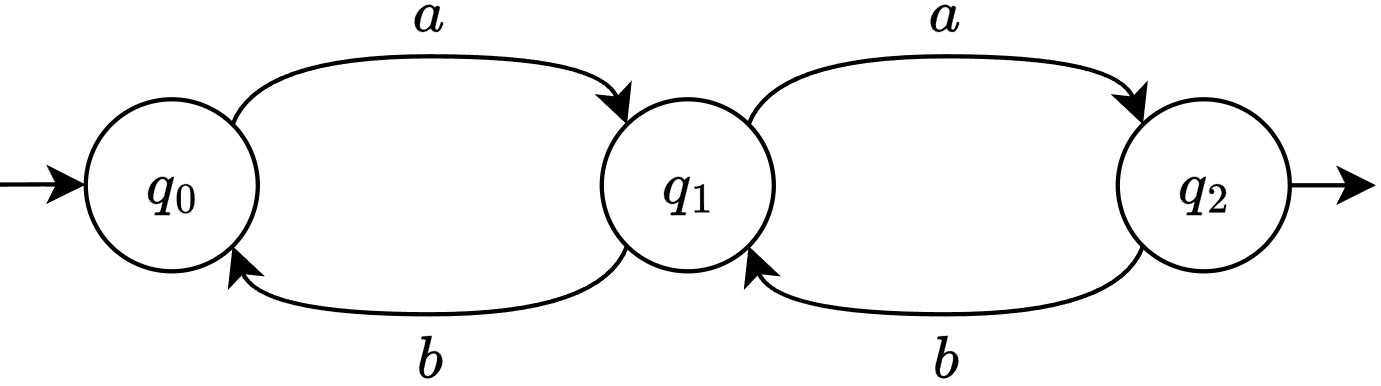
\includegraphics[width=0.5\linewidth]{images/compl.png}
    \end{figure}
    To obtain the complement automaton, introduce the error state $p$, resulting in the modified automaton:
    \begin{figure}[H]
        \centering
        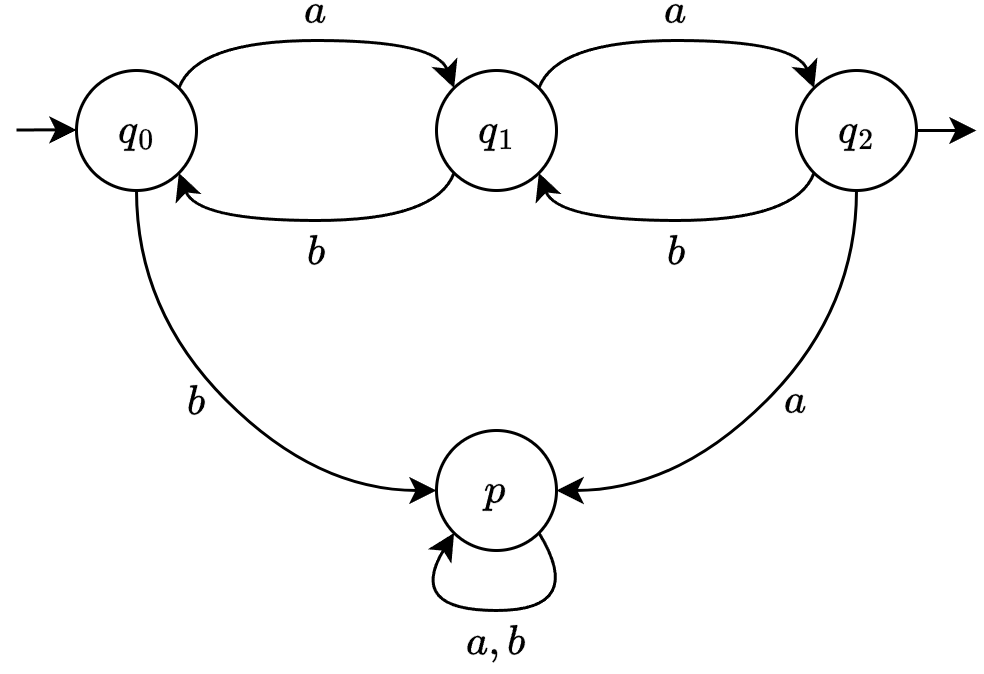
\includegraphics[width=0.5\linewidth]{images/compl1.png}
    \end{figure}
    Finally, interchange final and non-final states to achieve the complement automaton:
    \begin{figure}[H]
        \centering
        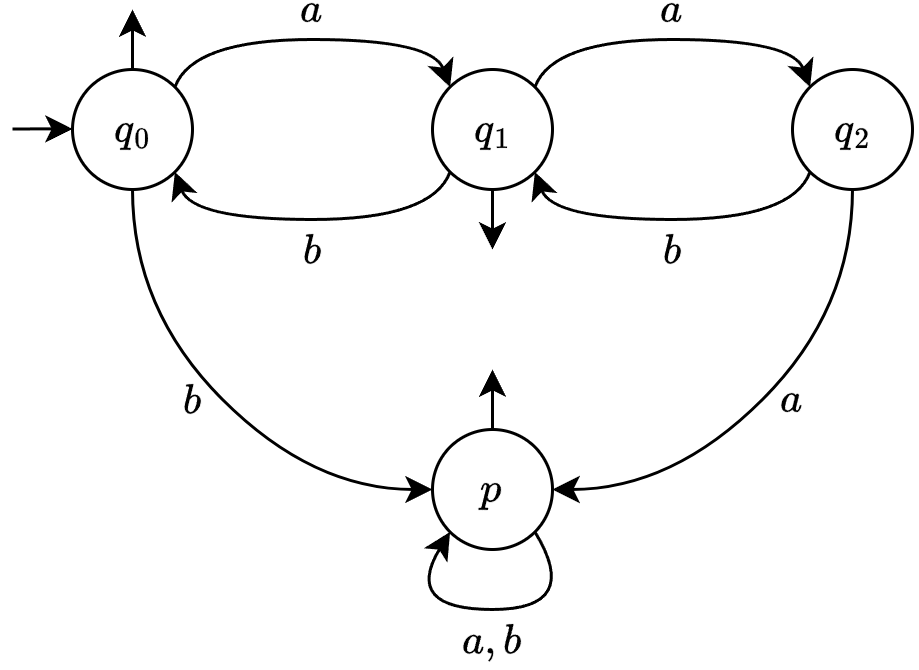
\includegraphics[width=0.5\linewidth]{images/compl2.png}
    \end{figure}
\end{example}
For the complement construction to function accurately, it is imperative that the original automaton be deterministic. 
Failure to meet this criterion may result in non-disjoint original and complement languages, violating the complement definition. 
Additionally, the complement automaton might encompass redundant states and may not be in its minimal form; hence, it should undergo reduction and minimization as needed.

\paragraph*{Cartesian product}
The product is a commonly used construction in formal languages, where a single automaton simulates the computation of two automata operating in parallel on the same input string. 
This construction is particularly valuable for building the intersection automaton. 
The steps to obtain the intersection automaton involve applying the De Morgan theorem:
\begin{enumerate}
    \item Construct deterministic recognizers for the two languages.
    \item Create the respective complement automata.
    \item Form their union using the Thompson construction.
    \item Transform the union automaton into a deterministic one using the Berry-Sethi construction.
    \item Apply complementation again to obtain the intersection automaton.
\end{enumerate}
Since the intersection of the two languages is directly recognized by the Cartesian product of their automata, obtaining the intersection automaton can be achieved more directly.
Assuming neither automaton contains spontaneous moves, the state set of the product machine is the Cartesian product of the state sets of the two automata. 
Each product state is a pair $\left\langle q^{\prime},q^{\prime\prime} \right\rangle $, where the left (right) member is a state of the first (second) machine.
The move is defined as follows:
\[\left\langle q^{\prime},q^{\prime\prime} \right\rangle \overset{a}{\rightarrow} \left\langle r^{\prime},r^{\prime\prime} \right\rangle \textnormal{ if and only if } q^{\prime} \overset{a}{\rightarrow} r^{\prime} \textnormal{ and } q^{\prime\prime} \overset{a}{\rightarrow} r^{\prime\prime}\]
The product machine has a move if and only if the projection of such a move onto the left (right) component is a move of the first (second) automaton. 
The initial and final state sets are the Cartesian products of the initial and final state sets of the two automata, respectively.
\begin{example}
    Consider the languages $L^{\prime}=(a\mid b)^{\ast}ab(a\mid b)^{\ast}$ and $L^{\prime\prime}=(a\mid b)^{\ast}ba(a\mid b)^{\ast}$. 
    The deterministic automaton for the language $L^{\prime}$ is illustrated below:
    \begin{figure}[H]
        \centering
        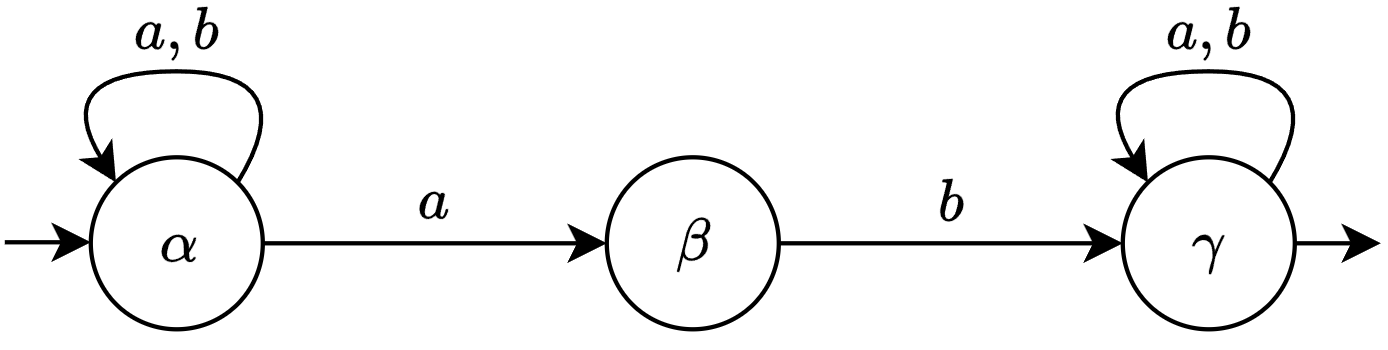
\includegraphics[width=0.5\linewidth]{images/int.png}
    \end{figure}
    Similarly, the deterministic automaton for the language $L^{\prime\prime}$ is depicted as follows:
    \begin{figure}[H]
        \centering
        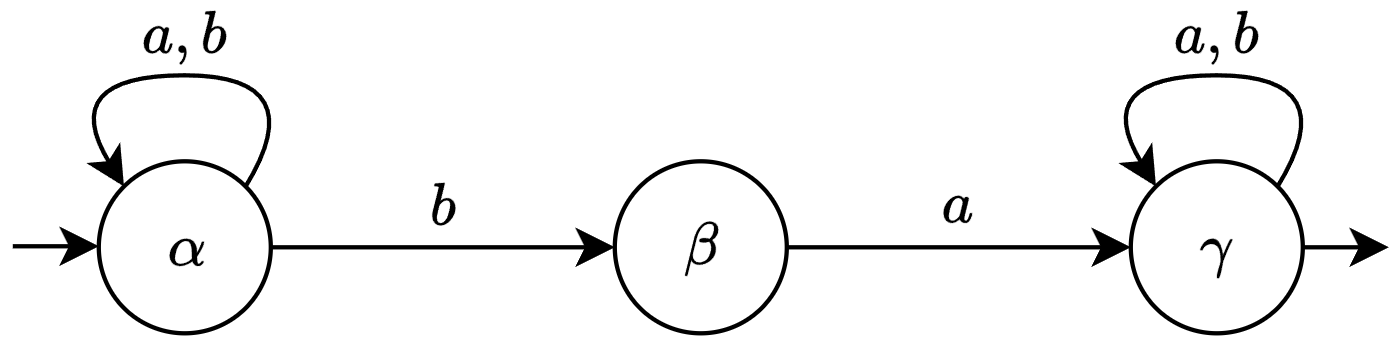
\includegraphics[width=0.5\linewidth]{images/int1.png}
    \end{figure}
    The intersection of these two languages is determined using the following table:
    \begin{figure}[H]
        \centering
        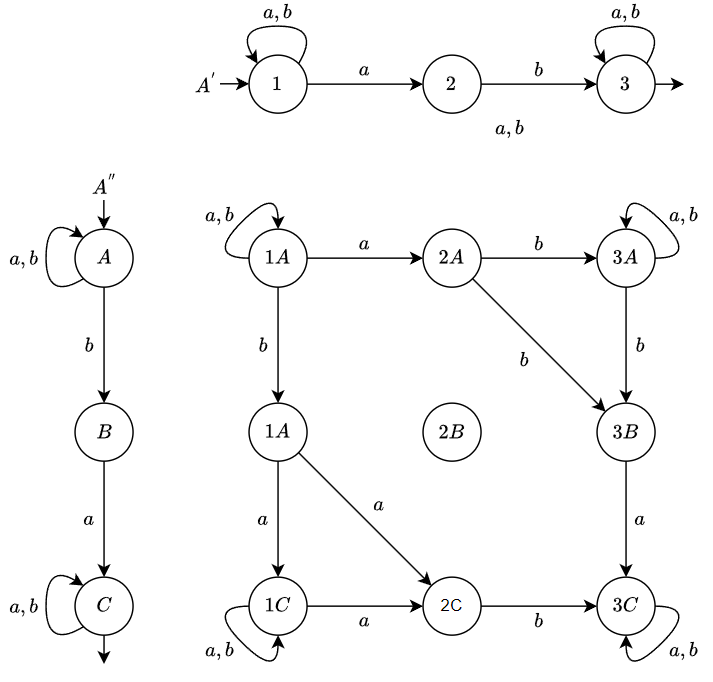
\includegraphics[width=0.65\linewidth]{images/int2.png}
    \end{figure}
\end{example}